% patterns.meta Hatch family only.
\usetikzlibrary{patterns.meta}

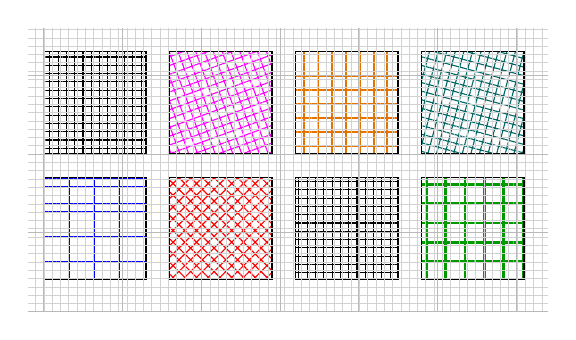
\begin{tikzpicture}[x=1cm,y=1cm]
  \path[draw,pattern={Hatch},pattern color=black] (0,0) rectangle +(1.3,1.3);
  \path[draw,pattern={Hatch[angle=20]},pattern color=magenta] (1.6,0) rectangle +(1.3,1.3);
  \path[draw,pattern={Hatch[distance=5pt,line width=.7pt]},pattern color=orange!90!black] (3.2,0) rectangle +(1.3,1.3);
  \path[draw,pattern={Hatch[angle=75]},pattern color=teal!80!black] (4.8,0) rectangle +(1.3,1.3);

  \path[draw,pattern={Hatch[xshift=1pt,yshift=1pt]},pattern color=blue] (0,-1.6) rectangle +(1.3,1.3);
  \path[draw,pattern={Hatch[angle=45,xshift=1pt,yshift=-1pt]},pattern color=red] (1.6,-1.6) rectangle +(1.3,1.3);
  \path[draw,pattern={Hatch[distance=3pt,line width=.4pt]},pattern color=black] (3.2,-1.6) rectangle +(1.3,1.3);
  \path[draw,pattern={Hatch[distance=7pt,line width=1pt]},pattern color=green!60!black] (4.8,-1.6) rectangle +(1.3,1.3);

  % Overlay reference grid for easier phase/offset comparison.
  \draw[step=3pt,gray!35,line width=.1pt] (-0.2,-2.0) grid (6.4,1.6);
  \draw[step=1cm,gray!55,line width=.16pt] (-0.2,-2.0) grid (6.4,1.6);
\end{tikzpicture}
